\documentclass[conference]{IEEEtran}

\usepackage{cite}
\usepackage{graphicx}
\graphicspath{{figs/}}
\DeclareGraphicsExtensions{.pdf,.jpg,.png}

\usepackage[caption=false,font=footnotesize]{subfig}
\usepackage{url}
\hyphenation{op-tical net-works semi-conduc-tor}


\begin{document}
%
% paper title
% can use linebreaks \\ within to get better formatting as desired
\title{Natural Interaction for Object Hand-Over [Video Abstract]}


\author{\IEEEauthorblockN{Mamoun Gharbi, Séverin Lemaignan, Jim Mainprice, Rachid Alami}
\IEEEauthorblockA{CNRS-LAAS, 7 av. du Colonel Roche\\
F-31077 Toulouse, France\\
Université de Toulouse, UPS, INSA, INP, ISAE, LAAS,\\
F-31077 Toulouse, France\\
Email: surname.name@laas.fr}
}
% make the title area
\maketitle


\begin{abstract}

The video presents in a didactic way several of the abilities and algorithms
required to achieve interactive "pick and place" tasks in a human environment.
Communication between the human and the robot relies on unconstrainted verbal
dialogue, the robot relies on multi-modal perception to track the human and its
environment, and implements real-time 3D motion planning algorithms to achieve
collision-free and human-aware interactive manipulation.

\end{abstract}


\section{The challenge of natural interactive manipulation}

\section{Main demonstrated abilities and algorithms}

The video demonstration is the result of the integration of many different
components. Besides {\it off the shelf} PR2 components (like the laser-based
localisation or the 2D navigation), we introduce here (figure~\ref{fig|archi})
several new components focuses on higher level planning and decision making.

\begin{figure}
        \centering
        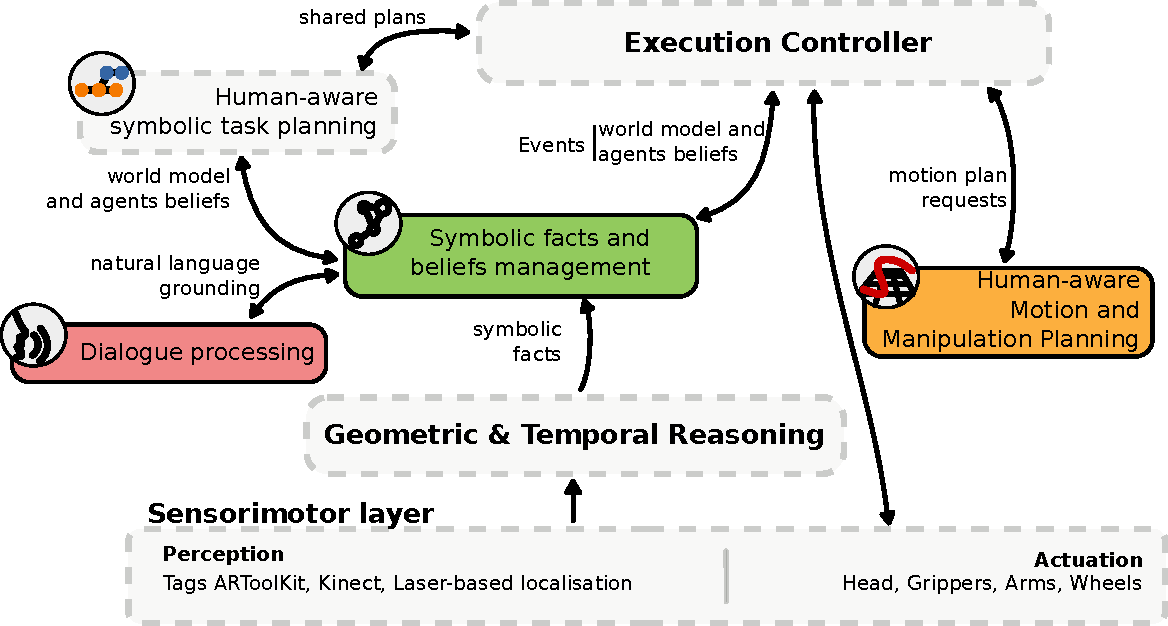
\includegraphics[width=0.9\columnwidth]{archi}
        \caption{Overview of the robot deliberative architecture. Coloured modules with plain borders are a specific focus of the video.}
        \label{fig|archi}
\end{figure}

\subsection{Symbolic modelling of the environment}



\subsection{Natural language processing}

\subsection{3D motion planning for manipulation}

\subsection{Human-aware trajectory planning for hand-over}

\section*{Acknowledgment}

This work has been partially funded by EU project SAPHARI.

\bibliographystyle{IEEEtran}
\bibliography{IEEEabrv,biblio}

% that's all folks
\end{document}


